%% Blinded submission manuscript
\documentclass[numbered,contemporary,mediumone]{oup-authoring-template}

\usepackage{booktabs}
\usepackage{multirow}
\usepackage{microtype}
\usepackage{placeins}
\usepackage{lineno}
\usepackage{setspace}

\setlength{\textfloatsep}{7pt plus 1pt minus 2pt}
\setlength{\floatsep}{7pt plus 1pt minus 2pt}
\setlength{\intextsep}{7pt plus 1pt minus 2pt}
\setlength{\abovecaptionskip}{3pt}
\setlength{\belowcaptionskip}{2pt}
\renewcommand{\topfraction}{0.95}
\renewcommand{\bottomfraction}{0.85}
\renewcommand{\textfraction}{0.05}
\renewcommand{\floatpagefraction}{0.80}
\doublespacing
\setcitestyle{numbers,square}

\providecommand{\authormark}[1]{\markboth{#1}{}}
\providecommand{\titlemark}[1]{\markright{#1}}
\makeatletter
\def\ps@opening{%
  \def\@oddhead{}%
  \def\@evenhead{}%
  \def\@oddfoot{\hfil\thepage\hfil}%
  \def\@evenfoot{\hfil\thepage\hfil}%
}
\makeatother

\journaltitle{BMC Bioinformatics}
\pubyear{2026}
\copyrightyear{2026}

\title[Temporal EC Prediction]{Dissecting Sequence, Structure, and Data Recency Effects
in Enzyme Commission Prediction under Temporal Distribution Shift}

\author[1,$\ast$]{Anonymous}
\address[1]{Affiliation blinded for review}
\corresp[$\ast$]{Corresponding author. Contact blinded for review.}

\abstract{%
\textbf{Background:}
Enzyme Commission (EC) prediction is increasingly evaluated with large protein
language models and structure-derived features, but headline benchmark scores
often conflate model architecture, training-set recency, sequence overlap,
label-vocabulary coverage, and temporal distribution shift. This makes it
difficult to determine whether a new representation improves biological
generalisation or mainly benefits from benchmark design.\\[3pt]
\textbf{Results:}
We analyze Contact-EC, a gated additive ESM-2/contact-map fusion model, as a controlled
probe for decomposing temporal EC prediction performance. On a Swiss-Prot 2023-01 temporal holdout
($N$\,=\,124, three seeds), fusion reaches Level-4 micro F1 of $0.6241\pm0.0170$,
outperforming ESM-2-only and contact-only baselines; topology perturbations indicate that
the contact-map encoder uses structural information beyond simple map-density cues. HIT-EC leads on this
one-year horizon (0.8471 vs.\ 0.6241), indicating that structure-aware fusion alone does
not close the short-horizon temporal gap. A larger SP-2024 temporal evaluation
($N$\,=\,1{,}226, three seeds) reveals a reversal under our mapped evaluation: HIT-EC falls to
$0.4578$ ($-$38.9\,pp) while Contact-EC improves to $0.6819\pm0.0026$ ($+$5.8\,pp),
yielding a $+$22.4\,pp advantage; a vocabulary-stratified analysis indicates that most of
HIT-EC's decrease is not explained by label-vocabulary mismatch. A Foldseek/TM-score-disjoint split shows that fusion
retains the highest micro F1 under explicit fold-level shift.\\[3pt]
\textbf{Conclusions:}
Contact-EC is best interpreted as a reproducible benchmark-decomposition
instrument rather than a replacement for curated homology transfer. The results
show that EC prediction benchmarks should explicitly report temporal cutoff,
sequence and fold relatedness, label-vocabulary coverage, data recency, and
whether the evaluation is closed-set or label-shifted.%
}

\keywords[Key words]{enzyme commission number; contact map; protein language model;
temporal evaluation; sequence--structure fusion; out-of-distribution generalisation}

\begin{document}
\maketitle
\thispagestyle{plain}
\pagestyle{plain}
\linenumbers

\section{Background}

Enzyme Commission (EC) numbers~\citep{mcdonald2023} provide a four-level hierarchy
for classifying enzyme-catalysed reactions, from broad reaction class to
substrate-specific function. Accurate EC assignment supports metabolic
reconstruction, pathway annotation, enzyme engineering, and drug-target
discovery, but experimental characterisation remains slow relative to the
growth of protein sequence databases.

Computational EC prediction has progressed from alignment-based
transfer~\citep{altschul1990} and 1D convolutional classifiers on one-hot
sequences~\citep{ryu2019,dalkiran2018} to large protein language model (PLM)
representations. ESM-2~\citep{lin2023} encodes residue-level evolutionary and
structural information from large sequence corpora, while systems such as
HIT-EC~\citep{dumontet2026}, CLEAN~\citep{yu2023}, EnzBert~\citep{buton2023},
and ECPick~\citep{han2024} apply hierarchical, contrastive, or evidential heads
to PLM embeddings. Structure-aware approaches derive contact-map features from
predicted structures~\citep{jumper2021,varadi2022}: DeepFRI~\citep{gligorijevic2021}
uses graph convolutional networks over residue contact graphs, and
CLEAN-Contact~\citep{ayres2024} integrates AlphaFold-derived maps into a
contrastive learning framework. ProteInfer~\citep{sanderson2023} further extends
function prediction with dilated convolutional sequence profiles. However,
reported scores are often obtained on same-distribution or near-contemporaneous
splits. This creates a reliability problem for biological deployment: a model
may rank highly because it has access to more recent annotations, an easier
closed-set label vocabulary, or near-duplicate sequences, rather than because
it generalises to newly annotated enzymes.

We study these factors using Contact-EC, a gated sequence--structure fusion model
combining ESM-2 650M embeddings with ResNet-50 contact-map features. The goal is
not to claim a new state-of-the-art EC predictor: HIT-EC remains stronger on the
shorter SP-2023-01 temporal holdout. Instead, Contact-EC is used as an instrument for benchmark
decomposition. We ask three questions that are central for journal-scale
model assessment. First, how different are same-distribution, sequence-disjoint,
and temporal EC evaluations? Second, do contact maps contribute signal
complementary to ESM-2 after controlling for topology-destroying perturbations?
Third, how much of temporal performance is explained by data recency,
closed-set label coverage, and fine-tuning strategy rather than by architecture alone?

Our analysis makes seven contributions. We provide a temporal label-shift audit for
Swiss-Prot 2023-01, separating 124 complete known-EC proteins from 344 partial or
novel-label cases. We show that contact maps alone match ESM-2 on hard
sequence-disjoint validation, while fusion improves temporal micro F1 over either
single modality. We test whether the contact branch uses fold topology rather than
contact-map density through shuffled, diagonal-only, and density-matched controls.
We add a Foldseek/TM-score-disjoint split to test structural generalisation beyond
sequence-disjoint evaluation. We extend temporal evaluation to SP-2024
($N$\,=\,1{,}226), observing a HIT-EC reversal under the mapped evaluation:
HIT-EC falls $-$38.9\,pp while
Contact-EC improves $+$5.8\,pp, and is higher than HIT-EC by $+$22.4\,pp
on the longer horizon, widening the modality gap from 17\,pp to 29\,pp. We decompose data recency and fine-tuning, finding that newer Swiss-Prot data helps
whereas end-to-end fine-tuning over-adapts. Finally, we translate these results
into reporting requirements for EC prediction studies: temporal cutoff, sequence
overlap, fold-level relatedness, label-vocabulary coverage, partial-label frequency, structure
availability, and whether each result is measured on a closed-set or label-shifted
benchmark.

\begin{figure}[!htbp]
\centering
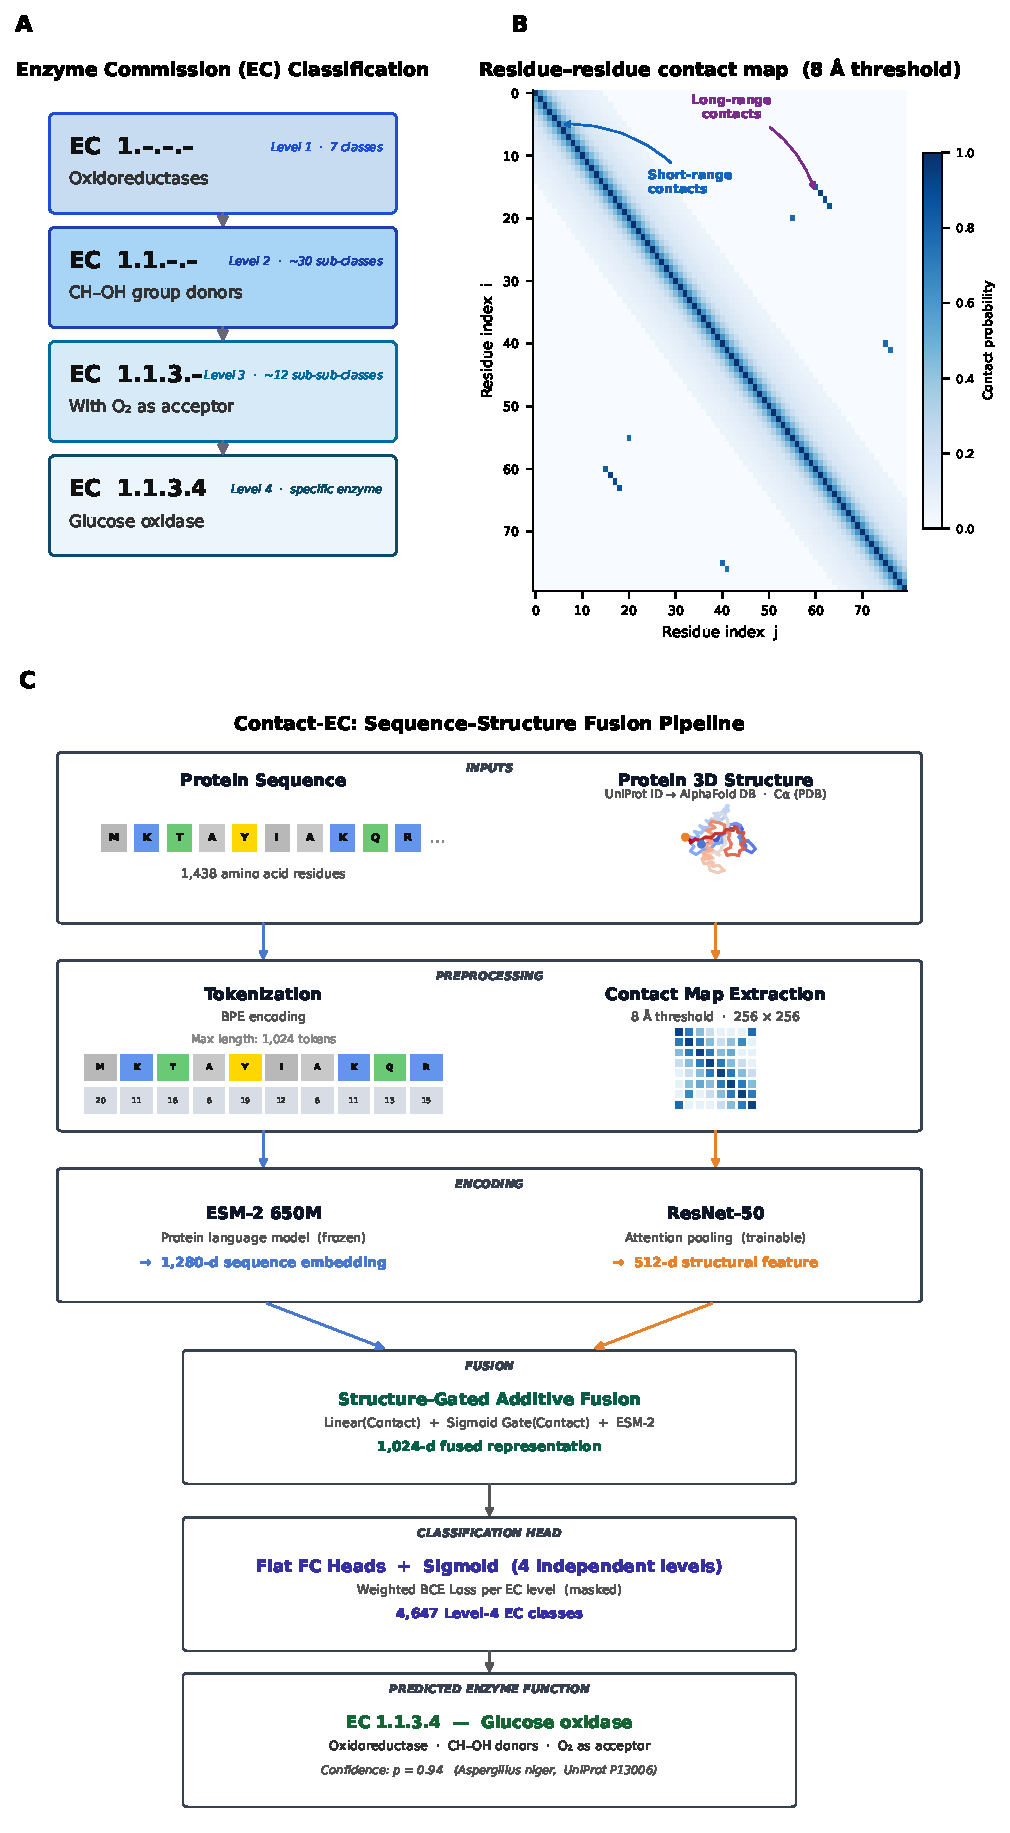
\includegraphics[height=0.89\textheight,keepaspectratio]{fig1_overview_print.pdf}
\caption{Contact-EC overview.
\textbf{(A)} EC number four-level hierarchy illustrated with glucose oxidase
(EC~1.1.3.4).
\textbf{(B)} Example protein contact map (8\,\AA{} threshold); short-range
backbone contacts form the diagonal band; long-range contacts (blue arrows)
encode tertiary fold topology.
\textbf{(C)} Contact-EC pipeline: ESM-2 (1280-d) and a ResNet-50 contact-map
encoder with attention pooling (512-d) are combined by structure-gated
additive fusion into a 1,024-d fused representation, then a flat FC $+$ sigmoid head
predicts all 4,647 Level-4 EC-Bench classes simultaneously (Contact-EC-Hier
replaces this head with a two-layer Transformer over four EC-level
tokens; Section~2.2).}
\label{fig:pipeline}
\end{figure}
\FloatBarrier

\section{Methods}

\subsection{Data and Splits}

The primary controlled experiments follow EC-Bench: Swiss-Prot February 2018 for
training (201{,}865 proteins after local preprocessing) and Swiss-Prot 2023-01 for
temporal testing. Sequences were truncated to 1{,}024 residues. AlphaFold
structures were retrieved from the AlphaFold Protein Structure Database~\citep{varadi2022} when
available; proteins without structures received zero contact maps. Contact maps
were built from C$\alpha$ distances using an 8\,\AA threshold, resized to
$256\times256$, and encoded in three channels: all contacts, short-range contacts
($|i-j|<12$), and long-range contacts ($|i-j|\geq12$).

We distinguish four evaluation regimes. A random 80/10/10 Swiss-Prot split measures
in-distribution performance. A MMSeqs2~\citep{steinegger2017} 30\% identity cluster split measures
sequence-disjoint generalisation. An EC-Bench-style hard validation set
(\texttt{val\_hard}; 6{,}247 proteins, $\leq$30\% sequence identity) provides a
shared validation protocol rather than an independent hidden test. Of 468
Swiss-Prot 2023-01 temporal proteins, only 124 have complete Level-4 EC labels
inside the SP-2018 vocabulary; the remaining 344 contain partial or novel labels.
A final temporal audit found no accession or exact-sequence overlap between these
124 proteins and either SP-2018 or ExpA training, but temporal evaluation alone
does not guarantee fold-disjointness.

To directly evaluate fold-level shift, we constructed an additional
Foldseek-disjoint split from the SP-2018 training corpus. Proteins with available
AlphaFold structures were clustered by Foldseek~\citep{vankempen2024} using TM-score threshold 0.50,
coverage 0.80, alignment type 1, cluster mode 1, and sensitivity 7.5. Cluster
assignment produced 170{,}573 training, 25{,}565 validation, and 16{,}725 test
proteins across 3{,}051/381/381 structure clusters, with zero protein-ID overlap
across partitions. This split is used only for the fold-disjoint audit and all
models are retrained on the corresponding training partition.

\subsection{Model}

The sequence branch uses ESM-2 650M~\citep{lin2023}
(\texttt{facebook/esm2\_t33\_650M\_UR50D}) and extracts the 1280-dimensional
\texttt{[CLS]} embedding. The structure branch applies a ResNet-50 encoder~\citep{he2016} with
attention pooling to the three-channel contact map and projects the output to 512
dimensions. The two representations are projected to a shared 1024-dimensional
space and combined by structure-gated additive fusion:
\[
\tilde{\mathbf{e}} = \phi(W_e\mathbf{e}), \qquad
\tilde{\mathbf{s}} = W_s\mathbf{s},
\]
\[
\mathbf{g} = \sigma(W_g\mathbf{s}),
\qquad
\mathbf{f} = \tilde{\mathbf{e}} + \mathbf{g}\odot W_a\tilde{\mathbf{s}}.
\]
The gate $\mathbf{g}$ is a function of the raw structure feature
$\mathbf{s}$ alone and is not conditioned on the sequence branch; $W_a$ is
implemented as a single-head attention layer applied to a single
structure token, which is mathematically equivalent to a learned linear
map, since softmax over one key is identically~1 regardless of the
query. This lets the gate learn to suppress an uninformative or missing
contact map without needing sequence context to detect it, giving
fallback behaviour to ESM-2-only performance.
Contact-EC-Hier passes the fused vector through a two-layer Transformer over four
EC-level tokens; the flat variant uses fully connected sigmoid outputs.
To audit whether this learned fusion block is necessary, we also train three
same-encoder flat-head controls: concatenation followed by an MLP, element-wise
summation, and a feature-wise gated MLP (Supplementary architecture-baseline
table).

\subsection{Training and Evaluation}

Models are trained with weighted binary cross-entropy across EC levels, with
weights $(0.1,0.1,0.2,0.6)$ for Levels 1--4 and masks for partial annotations.
Phase 1 trains downstream modules for 30 epochs with frozen ESM-2; Phase 2
partially unfreezes the final two ESM-2 blocks for 20 epochs at a lower learning
rate for Contact-EC-Hier. AdamW~\citep{loshchilov2019} with cosine annealing is used throughout, and checkpoints are selected
only on validation data. The main training recipe uses batch size 64, Phase-1
learning rate $10^{-3}$, Phase-2 learning rate $10^{-4}$, weight decay
$5\times10^{-4}$, dropout 0.3--0.4 depending on the split, 8\,\AA contact
thresholds, 256$\times$256 contact maps, and seeds 42/43/44 for repeated
temporal and Foldseek-disjoint comparisons (Supplementary training
hyper-parameter table). Level-4 micro F1 is the primary metric, with macro F1,
weighted F1, rare-EC F1, precision, and recall reported for interpretation.
Hyper-parameters were fixed before temporal testing.

\subsection{AI-assisted tools}

AI tools were used for grammar checking, LaTeX formatting assistance, and code
refactoring during manuscript preparation. All scientific content, experimental
design, analysis, and interpretation were performed by the author.

\section{Results}

\subsection{EC-Bench-Style Validation}

On EC-Bench \texttt{val\_hard}, the checkpoint-selected hard validation protocol,
contact maps alone reach nearly identical Level-4
micro F1 to ESM-2 650M (0.7650 vs.\ 0.7655; Table~\ref{tab:ecbench}). This parity
suggests that fold topology captures substantial EC-discriminative information
even without sequence embeddings. Fusion improves substantially: Contact-EC reaches
0.8879, while Contact-EC-Hier reaches 0.8698. Training dynamics in Supplementary
Fig.~S1 show that B3 converges within about 10 epochs and that fusion continues to
improve during partial unfreezing.

\begin{table}[!htbp]
\centering
\caption{EC-Bench hard validation results (\texttt{val\_hard}, 6{,}247 proteins,
$\leq$30\% identity), used for validation/checkpoint selection.}
\label{tab:ecbench}
\setlength{\tabcolsep}{5pt}
\begin{tabular}{lccc}
\toprule
Model & L4 Micro F1 & L4 Macro F1 & Best Epoch \\
\midrule
B1 (ESM-2, flat FC)       & 0.7655 & 0.1353 & 30 \\
B2 (ESM-2, hier.\ FC)     & 0.4204 & 0.0383 & 30 \\
B3 (Contact map only)     & 0.7650 & 0.1335 & 10 \\
Contact-EC (flat FC)      & \textbf{0.8879} & \textbf{0.2294} & 29 \\
Contact-EC-Hier           & 0.8698 & 0.2141 & 20 (Phase~2) \\
\bottomrule
\end{tabular}
\end{table}

\subsection{Temporal Label Shift}

The official Swiss-Prot 2023-01 temporal set contains 468 proteins, but only 124
are complete known-EC cases that can be scored within the SP-2018 closed-set label
space (Table~\ref{tab:labelshift}). The remaining 344 proteins expose an important
benchmark limitation: Level-4 closed-set scoring is undefined for incomplete
partial EC labels and cannot assign novel Level-4 classes outside the training
vocabulary. We therefore report main temporal
comparisons on the 124 evaluable proteins and use the full 468 proteins as a
label-shift audit. This separation is essential for interpreting temporal EC
prediction: a low score on all 468 proteins may reflect open-vocabulary label
shift rather than a failure to rank known EC classes, whereas a high score on the
124-protein subset may overstate deployability on newly annotated enzymes.
Supplementary hierarchical-prefix evaluation further shows that partial
annotations retain useful lower-level supervision and should not be counted as
Level-4 failures.

\begin{table}[!htbp]
\centering
\caption{Swiss-Prot 2023-01 label-shift audit. Partial annotations lack complete
Level-4 ground truth and are not assigned Level-4 F1.}
\label{tab:labelshift}
\setlength{\tabcolsep}{5pt}
\begin{tabular}{lrlc}
\toprule
Subset & $N$ & Interpretation & Closed-set L4 status \\
\midrule
Complete known EC labels & 124 & Main evaluable subset & Scored at L4 \\
Partial EC annotations   & 309 & Incomplete Level-4 labels & Not scored at L4 \\
Novel EC labels          & 35  & Outside SP-2018 vocabulary & Out of vocabulary \\
All temporal proteins    & 468 & Label-shift audit & Coverage audit \\
\bottomrule
\end{tabular}
\end{table}

\subsection{Temporal Performance}

On the complete temporal subset, sequence--structure fusion outperforms both
single-modality baselines (Table~\ref{tab:main}). Across three seeds, Contact-EC
improves micro F1 from 0.4508$\pm$0.0203 for B1 and 0.4244$\pm$0.0207 for B3 to
0.6241$\pm$0.0170. The 3B flat-fusion variant reaches 0.6316 in a single run, a
modest gain over the 650M fusion mean relative to the 4.5$\times$ parameter
increase. Contact-EC-Hier improves over single-modality baselines but
underperforms the flat head, mainly through lower recall. HIT-EC remains higher
at 0.8471, so we interpret Contact-EC as a decomposition model rather than a
replacement for stronger sequence-only systems.

Case-wise and baseline audits support this framing. Among 124 temporal proteins,
HIT-EC and Contact-EC both recover at least one correct EC for 63 proteins,
HIT-EC alone recovers 45, Contact-EC alone recovers 2, and both miss 14.
Changing the global threshold only modestly changes Contact-EC micro F1 (0.6032
at 0.5 versus 0.6167 at 0.65), and MMseqs2 top-hit EC transfer reaches 0.5852.
Trainable fusion controls remain below Contact-EC: concatenation reaches
0.5922$\pm$0.0150 micro F1, summation 0.5505$\pm$0.0230, and a gated MLP
0.5543$\pm$0.0525 (Supplementary architecture-baseline table).

\begin{table}[!htbp]
\centering
\caption{Temporal and external benchmark results. Swiss-Prot 2023-01 uses the
complete known-EC subset ($N$\,=\,124). B1, B3, and Contact-EC flat FC temporal
values are mean $\pm$ sample standard deviation across three seeds when shown;
other rows are single-run or externally reported. Bold denotes the best value among our
SP-2018-trained models. $^\dagger$ExpA is evaluated on the Level-4
encoder-evaluable intersection subset ($N$\,=\,99); Contact-EC trained on
SP-2018 reaches $0.6467\pm0.0210$ micro F1 on the same subset.}
\label{tab:main}
\scriptsize
\setlength{\tabcolsep}{3pt}
\begin{tabular}{lcccc}
\toprule
& \multicolumn{3}{c}{Swiss-Prot 2023-01} & Price-149 \\
\cmidrule(lr){2-4}\cmidrule(lr){5-5}
Model & Micro F1 & Weighted F1 & Rare-EC F1 & Micro F1 \\
\midrule
HIT-EC (own split)        & 0.930 & -- & -- & -- \\
HIT-EC (this test)        & 0.8471 & 0.8134 & 0.8322 & -- \\
CLEAN-Contact             & -- & -- & -- & 0.525 \\
\midrule
B1 (ESM-2, flat FC)       & $0.4508\pm0.0203$ & $0.3387\pm0.0194$ & $0.3292\pm0.0272$ & 0.0324 \\
B2 (ESM-2, hier.\ FC)     & 0.1111 & 0.0835 & 0.0000 & 0.0000 \\
B3 (Contact map only)     & $0.4244\pm0.0207$ & $0.3325\pm0.0237$ & $0.3354\pm0.0254$ & 0.0000 \\
Contact-EC (flat FC)      & $0.6241\pm0.0170$ & $0.5278\pm0.0222$ & $\mathbf{0.5257\pm0.0313}$ & 0.2500 \\
Contact-EC-Hier           & 0.5690 & 0.4528 & 0.3621 & 0.1263 \\
Contact-EC-3B (flat FC)   & \textbf{0.6316} & \textbf{0.5477} & 0.4786 & \textbf{0.2915} \\
\midrule
Contact-EC-ExpA (recent data)$^\dagger$ & $0.7417\pm0.0182$ & $0.6768\pm0.0168$ & $0.5474\pm0.0678$ & 0.2764 \\
Contact-EC-E2E (fine-tuned)   & 0.6703 & 0.6382 & 0.5091 & 0.2522 \\
\bottomrule
\end{tabular}
\end{table}

\begin{figure}[!htbp]
\centering

\includegraphics[width=\linewidth]{fig2_temporal_bars.pdf}
\caption{Level-4 micro F1 on two temporal holdouts.
\textbf{(A)} SP-2023-01 ($N$=124).
\textbf{(B)} SP-2024 ($N$=1,226).
Error bars: $\pm$1 s.d.\ across three training seeds (42/43/44); HIT-EC and
MMseqs2 are single deterministic runs. Contact-EC is the only neural model
that improves from Panel~A to Panel~B ($+$5.8\,pp), while HIT-EC regresses
$-$38.9\,pp.}
\label{fig:temporal_bars}
\end{figure}
\FloatBarrier

Bootstrap confidence intervals (1{,}000 resamples) confirm the main differences:
Contact-EC-3B [0.547, 0.711], Contact-EC [0.511, 0.686], Contact-EC-Hier
[0.476, 0.664], B1 [0.315, 0.521], and B3 [0.254, 0.473]. McNemar tests further
support Contact-EC over B1 ($\chi^2=22.4$, $p<0.001$) and over B3
($\chi^2=37.0$, $p<0.001$).
Supplementary late-fusion diagnostics show that simple post-hoc averaging or
maximum pooling of B1 and B3 probabilities does not reproduce the learned fusion
gain (best late-fusion temporal micro F1\,=\,0.4673 vs.\ 0.6032 for Contact-EC).
Retrained simple fusion baselines also remain lower than Contact-EC
(Supplementary architecture-baseline table).

\subsection{SP-2024 Larger Temporal Evaluation}

To verify that the fusion advantage holds at greater temporal scale, we constructed
a second temporal holdout from Swiss-Prot entries created after the SP-2023-01
release date. Applying the same closed-set filter---proteins with complete Level-4
EC labels inside the SP-2018 vocabulary---yields 1{,}226 evaluable proteins from
3{,}137 total new reviewed entries (39.1\% pass rate; the remaining 60.9\% carry
partial or novel EC labels, a label-shift fraction similar to SP-2023-01).

On SP-2024 ($N$\,=\,1{,}226, three seeds), the ESM-2-only baseline decreases:
B1 falls from $0.4508\pm0.0203$ to $0.3892\pm0.0121$ ($-$6.2\,pp). Contact-only
B3 is essentially stable ($0.4388\pm0.0166$, $+$1.4\,pp within seed variance),
while Contact-EC flat FC improves to $0.6819\pm0.0026$ ($+$5.8\,pp) and
Contact-EC-Hier to 0.6253 ($+$5.6\,pp) (Table~\ref{tab:sp2024}). The gap
between fusion and the ESM-2-only baseline widens from 17.3\,pp on SP-2023-01
to 29.3\,pp on SP-2024.

A MMseqs2 top-hit homology transfer baseline on SP-2024 achieves 0.7080
micro F1, a $+$12.3\,pp \emph{increase} over SP-2023-01 (0.5852), indicating
that SP-2024 proteins have sufficient homolog coverage in the SP-2018 training
set and are not intrinsically harder retrieval targets. Against this backdrop,
HIT-EC falls to 0.4578 on SP-2024 ($-$38.9\,pp), a decrease
substantially larger than any Contact-EC change. Contact-EC flat FC is consequently
higher than HIT-EC on SP-2024 by $+$22.4\,pp under this mapped evaluation, reversing the $-$22.3\,pp
deficit on SP-2023-01. This reversal is consistent with HIT-EC's sequence-only
architecture being sensitive to temporal distribution shift as the evaluation
horizon extends, while structural topology in Contact-EC may provide
complementary evidence not captured by sequence context alone. Bootstrap 95\,\% confidence
intervals (1{,}000 resamples, single-seed ecbench checkpoint) confirm
non-overlapping CIs between Contact-EC [0.6403, 0.6914] and both B1 [0.3520,
0.4117] and B3 [0.3051, 0.3643]; McNemar protein-level tests give
$\chi^2\!=\!327.6$ (CE vs B1) and $\chi^2\!=\!339.6$ (CE vs B3), both $p<0.0001$.

To test whether the HIT-EC decrease is explained by vocabulary
mismatch, we stratified SP-2024 proteins by whether their true Level-4
EC labels are covered by HIT-EC's 4{,}255-class vocabulary. Of 1{,}226
proteins, 1{,}000 (81.6\,\%) have \emph{all} true labels inside HIT-EC's
vocabulary (all\_in\_vocab), 29 (2.4\,\%) are partial, and 197 (16.1\,\%)
have no true label in HIT-EC's vocabulary (all\_out\_vocab).
On the all\_in\_vocab subset---where HIT-EC can in principle assign the
correct EC---HIT-EC achieves only 0.5496 micro F1, a $-$29.7\,pp drop
from its SP-2023-01 level of 0.8471. The vocabulary gap accounts for
roughly 9.2\,pp of the total $-$38.9\,pp decline; the remaining
$-$29.7\,pp (75\,\% of the total drop) remains after restricting to vocabulary-covered proteins.
Contact-EC is stable across all strata: 0.6965 on
all\_in\_vocab, 0.5000 on partial, and 0.5396 on all\_out\_vocab (Table~\ref{tab:vocab_strat}).

\begin{table}[!htbp]
\centering
\caption{SP-2024 temporal evaluation ($N$\,=\,1{,}226 complete known-EC
proteins from 3{,}137 new Swiss-Prot entries after 2023-01-25). B1, B3, and
Contact-EC (flat FC) values are mean\,$\pm$\,std across three seeds;
Contact-EC-Hier and HIT-EC are single-seed. HIT-EC decreases by $-$38.9\,pp
while Contact-EC improves, reversing the ranking seen on SP-2023-01 under this mapped evaluation.}
\label{tab:sp2024}
\setlength{\tabcolsep}{4pt}
\begin{tabular}{lccc}
\toprule
Model & SP-2023-01 & SP-2024 & $\Delta$ \\
\midrule
MMseqs2 (top-hit transfer) & 0.5852 & \textbf{0.7080} & $+$12.3\,pp \\
\midrule
B1 (ESM-2, flat FC)   & $0.4508\pm0.0203$ & $0.3892\pm0.0121$ & $-$6.2\,pp \\
B3 (Contact map only) & $0.4244\pm0.0207$ & $0.4388\pm0.0166$ & $+$1.4\,pp \\
Contact-EC (flat FC)  & $0.6241\pm0.0170$ & $\mathbf{0.6819\pm0.0026}$ & $+$5.8\,pp \\
Contact-EC-Hier       & 0.5690 & 0.6253 & $+$5.6\,pp \\
HIT-EC (mapped)       & 0.8471 & 0.4578 & $-$38.9\,pp \\
\bottomrule
\end{tabular}
\end{table}

\begin{figure}[!htbp]
\centering

\includegraphics[width=0.78\linewidth]{fig3_reversal_slope.pdf}
\caption{Model trajectories across the two temporal horizons. Each endpoint
value and signed change (pp) is annotated in the model's colour. HIT-EC
(red) falls $-$38.9\,pp, whereas Contact-EC (green) improves $+$5.8\,pp,
producing a $+$22.4\,pp reversal on SP-2024 (shaded region). Thick solid
lines: our model and HIT-EC; thin dashed lines: single-modality baselines.}
\label{fig:reversal}
\end{figure}

\begin{table}[!htbp]
\centering
\caption{HIT-EC vocabulary-stratified evaluation on SP-2024. Proteins are
grouped by whether their true Level-4 EC labels fall inside HIT-EC's
4{,}255-class vocabulary. Even among all\_in\_vocab proteins (where HIT-EC
can in principle succeed), HIT-EC drops $-$29.7\,pp from its SP-2023-01
level (0.8471), indicating that vocabulary mismatch alone does not explain the
observed HIT-EC decrease. Stratified Contact-EC values use the canonical
seed-42 checkpoint; therefore the aggregate score (0.6661) differs from the
three-seed mean in Table~\ref{tab:sp2024} (0.6819$\pm$0.0026).}
\label{tab:vocab_strat}
\setlength{\tabcolsep}{4pt}
\begin{tabular}{lrcc}
\toprule
Stratum & $N$ & HIT-EC F1 & Contact-EC F1 \\
\midrule
all\_in\_vocab  & 1{,}000 (81.6\,\%) & 0.5496 & \textbf{0.6965} \\
partial         &    29  (2.4\,\%)  & 0.1887 & \textbf{0.5000} \\
all\_out\_vocab &   197  (16.1\,\%) & 0.0000 & \textbf{0.5396} \\
\midrule
All             & 1{,}226           & 0.4578 & \textbf{0.6661} \\
\bottomrule
\end{tabular}
\end{table}
\FloatBarrier

\subsection{Foldseek-Disjoint Generalisation}

Sequence-disjoint evaluation does not necessarily remove structural fold
similarity. On the primary Foldseek/TM-score 0.50 split, all models show a large
absolute drop. Across three training seeds, the default Level-4 threshold of 0.5
gives micro F1 of $0.0433\pm0.0042$ for B1, $0.0400\pm0.0054$ for B3, and
$0.0872\pm0.0122$ for fusion. Validation-selected thresholds applied once to the
held-out Foldseek test split preserve the same ordering, with fusion reaching
$0.1685\pm0.0334$ micro F1 versus $0.0607\pm0.0009$ for B1 and
$0.0654\pm0.0016$ for B3. A single-seed TM-score sweep at 0.40/0.50/0.60 also
preserves the fusion advantage (0.2981/0.0998/0.4403 micro F1), although the
0.50 split has lower label coverage and a different cluster-assignment mode
(Supplementary Section~S9). In contrast, MMseqs2 top-hit EC transfer is much
stronger on the same split (Level-4 micro F1\,=\,0.5393), showing that this audit
tests complementary neural generalisation rather than replacement of curated
homology transfer.

The split also induces label-coverage shift: 31.5\% of positive Level-4 labels
in Foldseek test are absent from the corresponding training partition, and
31.6\% of test proteins contain at least one unseen Level-4 label. Among seen
labels, fusion is strongest for moderately represented classes (0.2484 micro F1
for 6--25 training proteins and 0.3278 for 26--100), indicating that
fold-disjoint performance reflects both structural shift and label-frequency
shift. A three-seed failure-mode audit further shows that fusion rescues 17.3\%
of Foldseek-test proteins missed by B1 and 12.5\% missed by B3; 11.0\% are
fusion-only rescues, whereas 41.9\% of all-model failures contain an unseen true
Level-4 label. When unseen positive labels are excluded from the same
Foldseek-disjoint prediction outputs, aggregate seen-label Level-4 micro F1
increases to 0.2159 for fusion versus 0.0863 for B1 and 0.0859 for B3
(Supplementary seen-label aggregate table), showing that the fusion advantage is
not solely a consequence of unseen-label composition.

\subsection{Topology Controls and Data Recency}

To test whether the contact branch uses topology rather than contact-map density or
length proxies, we evaluated three models under three perturbed contact-map variants on the
temporal test set ($N=124$): shuffled (symmetric row/column permutation, topology
destroyed), diagonal-only (constant band $|i-j|<12$, no protein-specific
long-range contacts), and density-matched random
(Table~\ref{tab:perturb}).

\begin{table}[!htbp]
\centering
\caption{Contact-map perturbation controls (temporal test, Swiss-Prot 2023-01,
$N=124$). B3 drops to zero under all perturbations.
Contact-EC flat FC decreases sharply ($-$54\,pp shuffled, $-$50\,pp random density),
consistent with reliance on fold topology rather than contact density alone.
Contact-EC-Hier shows negligible change: the structure gate routes to the ESM-2
branch when contact topology is destroyed, explaining why flat FC outperforms Hier.}
\label{tab:perturb}
\setlength{\tabcolsep}{5pt}
\begin{tabular}{lccc}
\toprule
Contact map variant & B3 & Contact-EC (flat FC) & Contact-EC-Hier \\
\midrule
Original                & 0.3646 & \textbf{0.6032} & 0.5690 \\
Shuffled (row/col perm.)& 0.0000 & 0.0625           & 0.5702 \\
Diagonal-only           & 0.0000 & 0.5242           & 0.5776 \\
Density-matched random  & 0.0000 & 0.0982           & 0.5641 \\
\bottomrule
\end{tabular}
\end{table}

\begin{figure}[!htbp]
\centering

\includegraphics[width=\linewidth]{fig4_perturbation.pdf}
\caption{Contact-map perturbation controls (SP-2023-01, $N$=124), shown
separately per model.
\textbf{(A)} B3 (contact-map only) drops to zero under all three
perturbations, consistent with strong sensitivity to contact-map topology and distribution.
\textbf{(B)} Contact-EC flat FC drops sharply under shuffling ($-$54.1\,pp)
and density-matched random ($-$50.5\,pp) but retains most performance under
diagonal-only ($-$7.9\,pp), indicating short-range secondary-structure
contacts remain informative.
\textbf{(C)} Contact-EC-Hier is invariant across all conditions ($\pm$1.0\,pp),
revealing that its structure gate routes to the ESM-2 branch when
topology is destroyed.}
\label{fig:perturbation}
\end{figure}
\FloatBarrier

Two findings emerge. First, the flat FC model exhibits massive degradation under
shuffling ($-$54.1\,pp) and random density matching ($-$50.5\,pp), confirming that
its performance derives from genuine three-dimensional fold topology rather than
contact-map density or protein-length proxies. The partial retention under
diagonal-only maps (0.5242, $-$7.9\,pp) indicates that short-range contacts
($|i{-}j|<12$, encoding secondary structure propensity) contribute substantially,
with long-range contacts providing an additional $+$7.9\,pp.
Second, Contact-EC-Hier is essentially invariant to perturbation ($\pm$0.9\,pp),
revealing that its structure gate has learned to route contact information to
zero when topology is disrupted---graceful degradation to ESM-2 performance.
This gate behaviour simultaneously explains why Contact-EC flat FC
\emph{outperforms} Contact-EC-Hier by 3.4\,pp on the temporal test: the
hierarchical Transformer head induces cross-level attention dynamics that
interfere with contact-branch integration, causing the gate to route
sub-optimally even on intact contact maps.

The recent-corpus experiment tests the effect of updating the training corpus and
label vocabulary. A recency-cutoff audit shows no accession or exact-sequence
overlap between the ExpA training split and the temporal proteins, but the ExpA
encoder evaluates only 99 of the 124 complete-known temporal proteins at Level 4.
On this matched $N=99$ intersection, Contact-EC trained on SP-2018 reaches
$0.6467\pm0.0210$ micro F1, whereas Contact-EC-ExpA reaches
$0.7417\pm0.0182$ across three seeds. Thus the fair-subset recent-corpus gain is
+9.5\,pp, not the naive +11.8\,pp obtained by
comparing different denominators. Sample size, class frequencies, label
coverage, and homolog coverage also change, so this is a recent-corpus effect
rather than a pure date effect. A separate MMseqs2 nearest-neighbour audit
supports this interpretation: on the same $N=99$ subset, moving from SP-2018 to
SP-2022/ExpA increases the median top-hit identity from 0.556 to 0.619, the
number of proteins with a $\geq0.60$-identity training neighbour from 38 to 49,
and top-hit exact Level-4 EC agreement from 69 to 78. In contrast,
end-to-end ESM-2 fine-tuning reaches similar in-distribution validation performance
but drops to 0.6703 temporally. This suggests over-adaptation of the PLM backbone
under limited supervised data and supports frozen or lightly tuned representations
for temporal robustness. The matched +9.5\,pp recent-corpus gain remains larger
than the +2.8\,pp gain from replacing ESM-2 650M with the 3B backbone,
reinforcing that benchmark date, data volume, homolog coverage, and label
coverage can matter as much as or more than backbone scale.

\section{Discussion}

The results support a nuanced interpretation. Contact maps provide a genuine
and complementary signal for EC prediction, especially on sequence-disjoint
validation, moderately represented fold-disjoint labels, and several broad EC
families. On the one-year horizon (SP-2023-01), the strongest temporal score
remains HIT-EC (0.8471), and controlled retraining shows that recent-corpus
factors explain a substantial part of the gap to Contact-EC (0.6241). This
distinction matters for method development: an architecture that improves a
fixed-date, closed-set benchmark may still underperform a simpler or sequence-only
system trained with a more recent label vocabulary.

Notably, the SP-2024 evaluation ($N$\,=\,1{,}226) complicates this picture in a
significant way. HIT-EC, which led by $+$22.3\,pp on SP-2023-01, falls to 0.4578
on SP-2024 ($-$38.9\,pp)---a decrease substantially larger than any Contact-EC
change. Contact-EC flat FC (0.6819\,$\pm$\,0.0026) consequently overtakes HIT-EC
by $+$22.4\,pp on SP-2024. A MMseqs2 top-hit transfer baseline achieves 0.7080 on SP-2024
($+$12.3\,pp over SP-2023-01), showing that SP-2024 proteins are not
intrinsically harder homology targets---the training corpus provides
adequate coverage. This makes HIT-EC's decrease more notable.
Vocabulary-stratified analysis (Table~\ref{tab:vocab_strat})
indicates that this decrease is not primarily an artefact of HIT-EC's smaller label
vocabulary: even among the 1{,}000 SP-2024 proteins (81.6\,\%) whose true EC labels
are fully inside HIT-EC's 4{,}255-class vocabulary, HIT-EC achieves only
0.5496---a $-$29.7\,pp drop from SP-2023-01. The vocabulary gap accounts
for only $\sim$9\,pp ($\sim$25\,\%) of the total $-$38.9\,pp decline; the
remaining $\sim$30\,pp persists in sequences that HIT-EC's vocabulary nominally covers.
Contact-EC maintains
strong performance across all vocabulary strata (0.6965, 0.5000, 0.5396 for
all\_in, partial, and all\_out proteins, respectively), consistent with structural
topology in Contact-EC providing evidence that may be complementary to sequence-derived features
and relatively stable across annual Swiss-Prot release cycles. These findings
suggest that structure-aware models may carry a temporal advantage at longer horizons
even when sequence-only models lead on shorter ones, and reinforce the case for
reporting evaluation horizon alongside headline benchmark scores.

The evaluation also shows why EC benchmark design matters. The same model can look
strong on random splits, near-parity on sequence-disjoint validation, and much
weaker under temporal shift. Moreover, the full Swiss-Prot 2023-01 temporal set is
not a single closed-set benchmark: 344/468 proteins contain partial or novel labels.
Future studies should report training cutoff, sequence overlap, fold-level
relatedness, label-vocabulary coverage, partial-label frequency, and structure availability alongside headline F1.
We recommend reporting both the evaluable closed-set subset and the full temporal
label-shift set, because these answer different questions: recognition of known EC
classes versus robustness to newly curated or incomplete annotations.

There are limitations. Contact-EC relies on AlphaFold or predicted structures, so
performance can degrade when external structures or predicted contact maps come
from a shifted distribution. On Price-149~\citep{price2018}, supplementary audit results show that
input coverage is available but exact Level-4 specificity drops sharply despite
stronger coarse-level EC recovery, indicating an OOD calibration and specificity
failure rather than a simple missing-input problem. A calibration audit supports
this interpretation: on Price-149, Contact-EC emits nonempty predictions for
51.5\% of encoded proteins with median top-1 probability 0.5527, but top-1
hit rate is only 27.9\%. Supplementary contact-pair and raw contact-map topology
nearest-neighbor audits further show high nearest training-set similarity for
nearly all evaluable temporal proteins, explaining why temporal results should
not be interpreted as fold-disjoint structural generalization. The explicit
Foldseek split addresses this issue, but it also exposes severe label-coverage
shift: in the primary 0.50 split, 31.5\% of Foldseek-test positive labels are
unseen in the corresponding training partition, compared with 15.9\% and 10.3\%
in the 0.40 and 0.60 sweep splits. MMseqs2 top-hit transfer remains
substantially stronger than all closed-set neural models, reinforcing that
Contact-EC is a decomposition probe rather than a homology replacement. Macro F1 remains low due to the long-tailed Level-4 label
space. The temporal test is small; although the main temporal B1/B3/Contact-EC
comparison, the matched recent-data audit, and the Foldseek audit now include
three-seed repeats, 3B and end-to-end variants are still single-run analyses due
to compute cost. Bootstrap and
paired tests therefore quantify sample-level uncertainty rather than definitive
rankings. Finally, supplementary open-vocabulary audits show that fusion confidence
can partially flag unseen-label cases, but closed-set models cannot solve novel EC
discovery without retrieval, abstention, or label-expansion mechanisms.

\section{Conclusions}

This study reframes structure-aware EC prediction as a benchmark decomposition
problem. Contact maps alone can match ESM-2 650M on hard sequence-disjoint
validation, and sequence--structure fusion substantially improves temporal F1 over
either modality alone. Perturbation controls indicate that the structure branch uses
fold topology, and Foldseek-disjoint evaluation shows that fusion retains a
measurable advantage under fold-level shift even though absolute closed-set
Level-4 performance remains low. Data-recency and fine-tuning controls show that annotation
cutoff and backbone adaptation strongly affect temporal performance. Critically,
an extended SP-2024 evaluation ($N$\,=\,1{,}226) shows that the published
sequence-only HIT-EC model decreases by $-$38.9\,pp over two-plus years while Contact-EC
holds and overtakes it under the mapped evaluation, suggesting that structure-aware
representations may provide complementary robustness as the temporal horizon grows. These findings
argue for EC prediction benchmarks that explicitly separate representation
generalisation from fold shift, label shift, data recency, backbone scale,
structure availability, and evaluation horizon.

\section*{Declarations}

\subsection*{Ethics approval and consent to participate}
Not applicable. This study uses publicly available protein sequence,
annotation, benchmark, and predicted-structure resources and does not involve
human participants, human data, human tissue, animals, or clinical intervention.

\subsection*{Consent for publication}
Not applicable.

\subsection*{Availability of data and materials}

Swiss-Prot sequences and EC annotations were downloaded from
UniProt~\citep{uniprot2023} (\url{https://www.uniprot.org}). AlphaFold structures were retrieved from the
AlphaFold Protein Structure Database (\url{https://alphafold.ebi.ac.uk}).
New-392 and Price-149 benchmark files are available from the CLEAN-Contact
repository~\citep{ayres2024}. EC-Bench training and test data can be obtained from the EC-Bench
GitHub repository~\citep{davoudi2026}. Code and reproducibility artifacts for reproducing tables
and figures are available at \url{https://github.com/jamesksh0130/contact-ec}.
Project name: Contact-EC. Project home page:
\url{https://github.com/jamesksh0130/contact-ec}. Archived version:
GitHub tag \texttt{bmc-submission-v1}. Operating system:
Linux. Programming language: Python. License: MIT. There are no restrictions
on non-academic use beyond the terms of the repository license and the licenses
of the underlying third-party datasets and models. At submission, the public
GitHub repository is the primary code and reproducibility archive.

\subsection*{Competing interests}
The author declares no competing interests.

\subsection*{Funding}
This research received no specific grant from any funding agency in the public,
commercial, or not-for-profit sectors.

\subsection*{Authors' contributions}
CRediT author statement: Author: Conceptualization, Methodology,
Software, Validation, Formal Analysis, Investigation, Data Curation,
Visualization, Writing -- Original Draft, Writing -- Review \& Editing.
The author has read and approved the final manuscript.

\subsection*{Acknowledgements}
The author acknowledges the developers and curators of UniProt, AlphaFold DB,
ESM, EC-Bench, CLEAN, CLEAN-Contact, and HIT-EC for making their resources
available to the research community.

\bibliographystyle{unsrtnat}
\bibliography{references}

\end{document}
